\documentclass{beamer}

\usepackage{beamerthemeCambridgeUS}
\usepackage[frenchb]{babel}
\usepackage[utf8]{inputenc}
\usecolortheme{beaver}

\usepackage{listings}
\usepackage{xcolor}
\lstdefinestyle{base}{
  basicstyle=\ttfamily\color{black} \footnotesize,
  moredelim=**[is][\color{blue}]{@}{@},
  moredelim=**[is][\color{red}]{&}{&}
}

% \setbeamertemplate{navigation symbols}{
% \insertframenumber/
% \inserttotalframenumber
% }

\usepackage{color}
\definecolor{vert}{rgb}{0,0.5,0}
\definecolor{violet}{rgb}{0.5,0,0.5}

\usepackage{tikz}
\usetikzlibrary{calc,positioning,matrix,arrows,shapes.geometric,shapes.symbols,shapes.misc,shapes,automata,petri,decorations.markings,shadows}
\usepackage{array}
\usepackage{subfig}

\usepackage[absolute,overlay]{textpos}
\usepackage{tcolorbox}

\usepackage[lined]{algorithm2e}
\usepackage{ulem}

%----------TIKZ
\usetikzlibrary{calc,arrows,shapes,automata,petri,positioning,decorations.markings,shadows}

\tikzset{
    use/.style={
    circle,draw=black,fill=black,scale=0.5,text=white
    },
    mpi/.style={
    rectangle,draw=black,fill=black,scale=0.8,text=white
    },
    provide/.style={
    circle,draw=black,fill=white,scale=0.5
    },
    component/.style={
    rectangle,rounded corners=3pt,draw=black
    },
    dcomponent/.style={
    rectangle,rounded corners=3pt,dashed,draw=black
    },
    progm/.style={rectangle,dotted, draw=black, thin, text width=8em, text centered,rounded corners, minimum height=2em},
  line/.style={draw, thin, ->, shorten >=2pt},
  purp/.style={rectangle, draw=violet,fill=violet!20, text width=10em, text centered,thin,rounded corners,inner sep=3pt},
  purp2/.style={rectangle, draw=violet,fill=violet!20, text width=15em, text centered,thin,rounded corners,inner sep=3pt},
  prog/.style={rectangle, draw=black, thin, text width=10em, text centered,rounded corners, minimum height=2em},
  progbl/.style={rectangle, draw=blue, thin, text width=10em, text centered,rounded corners, minimum height=2em},
  progrg/.style={rectangle, draw=red, thin, text width=10em, text centered,rounded corners, minimum height=2em},
  proggr/.style={rectangle, draw=vert, thin, text width=10em, text centered,rounded corners, minimum height=2em},
  progbrg/.style={rectangle, draw=red, very thick, text width=10em, text centered,rounded corners, minimum height=2em},
  progm/.style={rectangle,dotted, draw=black, thin, text width=10em, text centered,rounded corners, minimum height=2em},
  line/.style={draw, thin, ->, shorten >=2pt},
  inner/.style={rectangle, draw=blue!50,fill=blue!20, text width=10em, text centered,thin,rounded corners,inner sep=3pt},
  purp/.style={rectangle, draw=violet,fill=violet!20, text width=10em, text centered,thin,rounded corners,inner sep=3pt},
  purp2/.style={rectangle, draw=violet,fill=violet!20, text width=15em, text centered,thin,rounded corners,inner sep=3pt},
  purpb/.style={rectangle, draw=violet,fill=violet!20, text width=10em, text centered,very thick,rounded corners,inner sep=3pt},
  outer/.style={draw=vert,fill=green!20,thin,rounded corners,inner sep=10pt},
  outer2/.style={draw=vert,fill=green!20,text width=10em, text centered,thin,rounded corners,inner sep=3pt},
  outer3/.style={draw=red,fill=red!20, text width=10em, text centered,thin,rounded corners,inner sep=3pt},
  outer2b/.style={draw=vert,fill=green!20,text width=10em, text centered,very thick,rounded corners,inner sep=3pt},
  outer3b/.style={draw=red,fill=red!20, text width=10em, text centered,very thick,rounded corners,inner sep=3pt},
  comp/.style={draw=red,fill=red!20, text width=10em, text centered,thin,rounded corners,inner sep=10pt},
  the/.style={rectangle, draw=black, thin, text width=16em, text centered,rounded corners, minimum height=2em},
  the2/.style={rectangle,dotted, draw=black, thin, text centered,rounded corners, minimum height=2em},
  the3/.style={rectangle, draw=black, thin, text width=12em, text centered,rounded corners, minimum height=2em},
  the4/.style={rectangle,draw=black, thin, text centered,rounded corners, minimum height=2em},
}
%-------------
% * * * * * * * * * * * * * * *  ANNEXES * * * * * * * * * * * * * * * * * *
\newcommand{\backupbegin}{
   \newcounter{framenumberappendix}
   \setcounter{framenumberappendix}{\value{framenumber}}
}
\newcommand{\backupend}{
   \addtocounter{framenumberappendix}{-\value{framenumber}}
   \addtocounter{framenumber}{\value{framenumberappendix}} 
}

\AtBeginSection[]
{
  \begin{withoutheadline}
   \begin{frame}
   \frametitle{Table of contents}
        \tableofcontents[currentsection,hideallsubsections]
   \end{frame}
   \end{withoutheadline}
}
%-------------------------------------------------------------

\def\pprec{\mathrel{\scalebox{.9}[1]{$\prec$}\mkern-3mu%
  \scalebox{.4}[1]{$\prec$}\mkern-5.5mu\scalebox{.4}[1]{$\prec$}}}

\makeatletter
    \newenvironment{withoutheadline}{
        \setbeamertemplate{headline}[default]
        \def\beamer@entrycode{\vspace*{-\headheight}}
    }{}
\makeatother

%-------------------------------------------------------------------
\title[Journée Langages LIP]{The Multi-Stencil Language}
\author[Hélène Coullon]{\underline{Hélène Coullon}, Christian Perez and Julien Bigot}
\institute[Inria]{Inria Avalon, LIP Lyon}
\date[$17^{th}$ March 2016]{$17^{th}$ March 2016\\Journée Langages du LIP}
%-------------------------------------------------------------------

\begin{document}

%---------------
%---------------
\begin{withoutheadline}

\begin{frame}
    \titlepage
\end{frame}

% INTRODUCTION / MOTIVATION
%--------
%----------
\begin{frame}
\frametitle{High performance computing and parallelism in 2015}
\begin{center}
\only<1>{
  \begin{tikzpicture}
    \matrix[row sep=0.6cm,column sep=0.5cm] {
      \node[progbl] (para) {Parallel\\Programming models}; \\
      \node[progrg] (mod) {Parallel libraries\\ and languages};\\
      \node[proggr] (exec) {Hardware};\\
    };

    \node[fill=white,right of=exec,node distance=3cm] (grap) {\scriptsize \textcolor{vert}{Clusters}};
    \node[fill=white,right of=grap,node distance=2cm] (mc) {\scriptsize \textcolor{vert}{Multi-cores}};
    \node[fill=white,right of=mc,node distance=2cm] (gpu) {\scriptsize \textcolor{vert}{GPGPUs}};
    \node[fill=white,right of=gpu,node distance=2cm] (many) {\scriptsize \textcolor{vert}{Many-cores ...}};

    \begin{scope} [every path/.style=line]
      \path (para) -- (mod);
      \path (mod) -- (exec);

      \path (grap) edge[->,thin, bend right=50] (mc);
      \path (grap) edge[->,thin, bend right=50] (gpu);
      \path (grap) edge[->,thin, bend right=50] (many);
    \end{scope}
  \end{tikzpicture}
}
%--------
\only<2>{
  \begin{tikzpicture}
    \matrix[row sep=0.6cm,column sep=0.5cm] {
      \node[progbl] (para) {Parallel\\Programming models}; \\
      \node[progrg] (mod) {Parallel libraries\\ and languages};\\
      \node[proggr] (exec) {Hardware};\\
    };

    \node[fill=white,right of=exec,node distance=3cm] (grap) {\scriptsize \textcolor{vert}{Clusters}};
    \node[fill=white,right of=grap,node distance=2cm] (mc) {\scriptsize \textcolor{vert}{Multi-cores}};
    \node[fill=white,right of=mc,node distance=2cm] (gpu) {\scriptsize \textcolor{vert}{GPGPUs}};
    \node[fill=white,right of=gpu,node distance=2cm] (many) {\scriptsize \textcolor{vert}{Many-cores ...}};

    \node[fill=white,right of=para,node distance=3.5cm] (donn) {\scriptsize \textcolor{blue}{Data parallelism}};
    \node[fill=white,right of=donn,node distance=2.7cm] (tach) {\scriptsize \textcolor{blue}{Task parallelism}};
    \node[fill=white,right of=tach,node distance=2.7cm] (mess) {\scriptsize \textcolor{blue}{Message passing ...}};

    \begin{scope} [every path/.style=line]
      \path (para) -- (mod);
      \path (mod) -- (exec);

      \path (grap) edge[->,thin, bend right=50] (mc);
      \path (grap) edge[->,thin, bend right=50] (gpu);
      \path (grap) edge[->,thin, bend right=50] (many);
    \end{scope}
  \end{tikzpicture}
}
%--------
\only<3>{

  \begin{tikzpicture}
    \matrix[row sep=0.6cm,column sep=0.5cm] {
      \node[progbl] (para) {Parallel\\Programming models}; \\
      \node[progrg] (mod) {Parallel libraries\\ and languages};\\
      \node[proggr] (exec) {Hardware};\\
    };

    \node[fill=white,right of=exec,node distance=3cm] (grap) {\scriptsize \textcolor{vert}{Clusters}};
    \node[fill=white,right of=grap,node distance=2cm] (mc) {\scriptsize \textcolor{vert}{Multi-cores}};
    \node[fill=white,right of=mc,node distance=2cm] (gpu) {\scriptsize \textcolor{vert}{GPGPUs}};
    \node[fill=white,right of=gpu,node distance=2cm] (many) {\scriptsize \textcolor{vert}{Many-cores ...}};

    \node[fill=white,right of=para,node distance=3.5cm] (donn) {\scriptsize \textcolor{blue}{Data parallelism}};
    \node[fill=white,right of=donn,node distance=2.7cm] (tach) {\scriptsize \textcolor{blue}{Task parallelism}};
    \node[fill=white,right of=tach,node distance=2.7cm] (mess) {\scriptsize \textcolor{blue}{Message passing ...}};
  
    \node[fill=white,right of=mod,node distance=3cm] (bsp) {\scriptsize \textcolor{red}{BSP}};
    \node[fill=white,right of=bsp,node distance=1.5cm] (mpi) {\scriptsize \textcolor{red}{MPI}};
    \node[fill=white,right of=mpi,node distance=1.5cm] (openmp) {\scriptsize \textcolor{red}{OpenMP}};
    \node[fill=white,right of=openmp,node distance=1.5cm] (cuda) {\scriptsize \textcolor{red}{Cuda}};
    \node[fill=white,right of=cuda,node distance=1.5cm] (opencl) {\scriptsize \textcolor{red}{OpenCL ...}};

    \begin{scope} [every path/.style=line]
      \path (para) -- (mod);
      \path (mod) -- (exec);

      \path (grap) edge[->,thin, bend right=50] (mc);
      \path (grap) edge[->,thin, bend right=50] (gpu);
      \path (grap) edge[->,thin, bend right=50] (many);
      \path (mpi) edge[->,thin, bend right=50] (openmp);
      \path (mpi) edge[->,thin, bend right=50] (cuda);
      \path (bsp) edge[->,thin, bend right=50] (mpi);
    \end{scope}

  \end{tikzpicture}
}
%--------
\only<4>{
  \begin{tikzpicture}
    \matrix[row sep=0.6cm,column sep=0.5cm] {
      \node[progbl] (para) {Parallel\\Programming models}; \\
      \node[progrg] (mod) {Parallel libraries\\ and languages};\\
      \node[proggr] (exec) {Hardware};\\
    };

    \node[fill=white,right of=exec,node distance=3cm] (grap) {\scriptsize \textcolor{vert}{Clusters}};
    \node[fill=white,right of=grap,node distance=2cm] (mc) {\scriptsize \textcolor{vert}{Multi-cores}};
    \node[fill=white,right of=mc,node distance=2cm] (gpu) {\scriptsize \textcolor{vert}{GPGPUs}};
    \node[fill=white,right of=gpu,node distance=2cm] (many) {\scriptsize \textcolor{vert}{Many-cores ...}};

    \node[fill=white,right of=para,node distance=3.5cm] (donn) {\scriptsize \textcolor{blue}{Data parallelism}};
    \node[fill=white,right of=donn,node distance=2.7cm] (tach) {\scriptsize \textcolor{blue}{Task parallelism}};
    \node[fill=white,right of=tach,node distance=2.7cm] (mess) {\scriptsize \textcolor{blue}{Message passing ...}};
  
    \node[fill=white,right of=mod,node distance=3cm] (bsp) {\scriptsize \textcolor{red}{BSP}};
    \node[fill=white,right of=bsp,node distance=1.5cm] (mpi) {\scriptsize \textcolor{red}{MPI}};
    \node[fill=white,right of=mpi,node distance=1.5cm] (openmp) {\scriptsize \textcolor{red}{OpenMP}};
    \node[fill=white,right of=openmp,node distance=1.5cm] (cuda) {\scriptsize \textcolor{red}{Cuda}};
    \node[fill=white,right of=cuda,node distance=1.5cm] (opencl) {\scriptsize \textcolor{red}{OpenCL ...}};

    \begin{scope} [every path/.style=line]
      \path (para) -- (mod);
      \path (mod) -- (exec);

      \path (grap) edge[->,thin, bend right=50] (mc);
      \path (grap) edge[->,thin, bend right=50] (gpu);
      \path (grap) edge[->,thin, bend right=50] (many);
      \path (mpi) edge[->,thin, bend right=50] (openmp);
      \path (mpi) edge[->,thin, bend right=50] (cuda);
      \path (bsp) edge[->,thin, bend right=50] (mpi);

      \path (mpi) -- (donn);
      \path (mpi) -- (tach);
      \path (mpi) -- (mess);
      \path (bsp) -- (donn);
      \path (bsp) -- (mess);
      \path (openmp) -- (tach);
      \path (openmp) -- (donn);
      \path (cuda) -- (tach);
      \path (opencl) -- (tach);
      \path (opencl) -- (mess);
    \end{scope}
  \end{tikzpicture}
}
%---------
\only<5>{
  \begin{tikzpicture}
    \matrix[row sep=0.6cm,column sep=0.5cm] {
      \node[progbl] (para) {Parallel\\Programming models}; \\
      \node[progrg] (mod) {Parallel libraries\\ and languages};\\
      \node[proggr] (exec) {Hardware};\\
    };

    \node[fill=white,right of=exec,node distance=3cm] (grap) {\scriptsize \textcolor{vert}{Clusters}};
    \node[fill=white,right of=grap,node distance=2cm] (mc) {\scriptsize \textcolor{vert}{Multi-cores}};
    \node[fill=white,right of=mc,node distance=2cm] (gpu) {\scriptsize \textcolor{vert}{GPGPUs}};
    \node[fill=white,right of=gpu,node distance=2cm] (many) {\scriptsize \textcolor{vert}{Many-cores ...}};

    \node[fill=white,right of=para,node distance=3.5cm] (donn) {\scriptsize \textcolor{blue}{Data parallelism}};
    \node[fill=white,right of=donn,node distance=2.7cm] (tach) {\scriptsize \textcolor{blue}{Task parallelism}};
    \node[fill=white,right of=tach,node distance=2.7cm] (mess) {\scriptsize \textcolor{blue}{Message passing ...}};
  
    \node[fill=white,right of=mod,node distance=3cm] (bsp) {\scriptsize \textcolor{red}{BSP}};
    \node[fill=white,right of=bsp,node distance=1.5cm] (mpi) {\scriptsize \textcolor{red}{MPI}};
    \node[fill=white,right of=mpi,node distance=1.5cm] (openmp) {\scriptsize \textcolor{red}{OpenMP}};
    \node[fill=white,right of=openmp,node distance=1.5cm] (cuda) {\scriptsize \textcolor{red}{Cuda}};
    \node[fill=white,right of=cuda,node distance=1.5cm] (opencl) {\scriptsize \textcolor{red}{OpenCL ...}};

    \begin{scope} [every path/.style=line]
      \path (para) -- (mod);
      \path (mod) -- (exec);

      \path (grap) edge[->,thin, bend right=50] (mc);
      \path (grap) edge[->,thin, bend right=50] (gpu);
      \path (grap) edge[->,thin, bend right=50] (many);
      \path (mpi) edge[->,thin, bend right=50] (openmp);
      \path (mpi) edge[->,thin, bend right=50] (cuda);
      \path (bsp) edge[->,thin, bend right=50] (mpi);

      \path (mpi) -- (donn);
      \path (mpi) -- (tach);
      \path (mpi) -- (mess);
      \path (bsp) -- (donn);
      \path (bsp) -- (mess);
      \path (openmp) -- (tach);
      \path (openmp) -- (donn);
      \path (cuda) -- (tach);
      \path (opencl) -- (tach);
      \path (opencl) -- (mess);
      
      \path (mpi) -- (grap);
      \path (mpi) -- (mc);
      \path (mpi) -- (many);
      \path (bsp) -- (grap);
      \path (bsp) -- (mc);
      \path (cuda) -- (gpu);
      \path (openmp) -- (many);
      \path (openmp) -- (mc);
      \path (opencl) -- (gpu);
      \path (opencl) -- (mc);
      \path (opencl) -- (many);
      \path (opencl) -- (grap);
    \end{scope}

  \end{tikzpicture}

  \medskip
  \textit{Very complex domain !}
}
  \end{center}
\end{frame}
%----------
%-------------------------------------------------------------
\begin{frame}
\frametitle{"Please Help"}
%implicitly parallel (one sep. of concerns) / specific / performance
\begin{block}{HPC}
\begin{itemize}
\item Heterogenous and complex parallel hardware
\item Many programming models to combine
\item Expert programming
\end{itemize}
\end{block}

\begin{block}{Users}
Weather, climat, physics, biology etc.
\end{block}

\begin{center}
Separation of concerns between domain/parallelization and optimization\\
Domain specific languages (DSL)\\
\medskip
\resizebox{2cm}{!}{\includegraphics{images/scientist.jpg}}
\end{center}
\end{frame}
%-------------------------------------------------------------
\begin{frame}
\frametitle{Contribution}
%implicitly parallel (one sep. of concerns) / specific / performance
\begin{block}{From MSL}
\begin{itemize}
\item Descriptive language,
\item for Multi-Stencil simulations,
\item without numerical code.
\end{itemize}
\end{block}

\begin{block}{To}
\begin{itemize}
\item Parallel pattern of the simulation,
\item with automatic synchronizations for data and task parallelism,
\item with empty functions to fill,
\item with good performance.
\end{itemize}
\end{block}

Separation of concerns between domain/implementation/parallelization

\end{frame}
%-------------------------------------------------------------


% presentation of the table of contents
%-------------------------------------------------------------
\begin{frame}
\frametitle{Table of contents}
    \tableofcontents[hideallsubsections]
\end{frame}
%-------------------------------------------------------------

\end{withoutheadline}

%-------------------------------------------------------------
\section{The domain: Multi-Stencil}
%-------------------------------------------------------------
\begin{frame}
\frametitle{What is a multi-stencil simulation ?}
\begin{center}
\begin{tikzpicture}
\def \n {5}
\def \radius {3cm}
\def \margin {8} % margin in angles, depends on the radius

  \node[purp2,align=center] (edp) at ({360/\n * (2 - 1)}:\radius) {set of PDEs\\\scriptsize $\frac{\partial u(x,y,t)}{\partial t} = \frac{\partial^2 u(x,y,t)}{\partial x^2} + \frac{\partial^2 u(x,y,t)}{\partial y^2}$};
  \node[rectangle,dotted, draw=black, thin, text width=7em, text centered,rounded corners, minimum height=2em,align=center,right of=edp,node distance=6cm] (cond) {\tiny Behavior of the phenomena\\and boundary behaviors};
  \path[line,dotted] (edp) -- (cond);
  \node[purp,align=center] (maillage) at ({360/\n * (1 - 1)}:\radius) {Mesh and\\time iterations};
  \path[->] (maillage) edge[<-,thin,shorten <=2pt,shorten >=2pt, bend right=40]  node [fill=white,align=center] {\scriptsize Discretization} (edp.east);
  \path[] (edp.west) edge[thin,shorten <=2pt,shorten >=2pt, bend right=90]  node [draw,circle,fill=white] (plus) {\scriptsize +} (maillage.west);
  \node[purp,align=center, below of=plus, node distance=3cm] (sche) {Numerical schemes\\Explicit = \textcolor{red}{stencil}};
  \node[fill=white,right of=sche,node distance=6cm,align=left] {\tiny Quantity $\sigma(x,t)$ computed from quantities at $(x,t)$ if different,\\\tiny $(x,t-1)$ and $(y,t-1)$, where $y$ is a neighborhood of $x$};
  \path[line] (plus) -- node [fill=white,align=center] {\scriptsize Numerical methods\\\scriptsize Finite difference/volume/elements} (sche);
\end{tikzpicture}
\end{center}
\end{frame}
%-------------------------------------------------------------
\begin{frame}
\frametitle{Multi-Stencil algorithm}
\begin{algorithm}[H]
 Create the mesh $\mu$\\
 Create the quantities to simulate mapped onto $\mu$\\
 Initialization of the quantities and parameters\\
 Create the time step $\delta t$\\
 Create the maximum time $tmax$\\
 \While{$criteria(t)==true$}{
 \For{each element of the boundary}{
   Numerical computations of boundary conditions
 }
  \For{each $x \in \mu$}{
  Compute stencils and auxiliary computations
  }
  $t = t+\delta t$
 }
 ...
\end{algorithm}
\end{frame}
%-------------------------------------------------------------
\begin{frame}
\frametitle{Definitions}
\begin{block}{Mesh}
\begin{itemize}
\item \textit{Mesh}: graph without bridges
\item \textit{Mesh entity}: sub-graph of the mesh
\item \textit{Group of mesh entities}: set of mesh entities of the same type
\item \textit{Computation domain}: sub-part of a group
\item \textit{Neighboorhood}: function from a mesh entity to a set of mesh entities (possibly from a different group than the input)
\end{itemize}
\end{block}

\begin{block}{Quantities}
\begin{itemize}
\item A \textit{quantity} is mapped onto a group of mesh entities
\item A \textit{scalar} is global to the simulation and is typically a numerical value constant or not
\end{itemize}
\end{block}
\end{frame}
%-------------------------------------------------------------
\begin{frame}
\frametitle{Definitions}
\begin{block}{Time and computations}
\begin{itemize}
\item \textit{Time}: time step and convergence criteria
\item \textit{Computation}:
\begin{itemize}
\item Set of scalar read
\item Set of quantities read, on which neighborhood
\item Quantity written, on which computation domain
\item A numerical expression
\end{itemize}
\end{itemize}
\end{block}

\begin{block}{Four kinds of computations}
\begin{itemize}
\item \textit{Stencil computation}: it exists a quantity read with a neighborhood
\item \textit{Boundary computation}: it exists a quantity read equal to the quantity written with a neighborhood
\item \textit{Local computation}: for all quantity read, there is not neighborhood
\item \textit{Reduction}: the quantity written is a scalar
\end{itemize}
\end{block}

\begin{equation*}
\mathcal{MSP}(\mathcal{M},\mathcal{E},\mathcal{D},\mathcal{N},\Delta,\mathcal{S},T,\Gamma)
\end{equation*}
\end{frame}
%-------------------------------------------------------------
\begin{frame}
\frametitle{Wait a while}
One can notice that
\begin{itemize}
\item Definitions independant of the mesh topology
\item Definitions independant of the numerical expression of computations
\end{itemize}
\begin{block}{The Multi-Stencil Language}
\begin{itemize}
\item Descriptive language mesh-agnostic and without numerical code asked to the user
\item Separation of concerns: description / implementation / parallelization
\end{itemize}
\end{block}
\end{frame}
%-------------------------------------------------------------

%-------------------------------------------------------------
\section{The Multi-Stencil Language}
%-------------------------------------------------------------
\begin{frame}[fragile]
\frametitle{The MSL language: the mesh}
\begin{center}
\resizebox{6cm}{!}{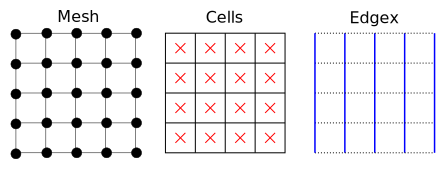
\includegraphics{images/mesh.pdf}}
\end{center}
\begin{columns}
\begin{column}{6.5cm}
\begin{lstlisting}[frame=single]
mesh : cart
mesh entities : cell, edgex
computation domains :
  d1 in cell
  d2 in edgex
stencil shapes : 
  ncc from cell to cell
  nce from cell to edgex
  nec from edgex to cell
\end{lstlisting}
\end{column}
\begin{column}{5.5cm}
\begin{itemize}
\item A cartesian mesh is used
\item Two kind of mesh entities are declared onto it
\item Two computations domains, one for each entity type
\item Three stencil shapes (neighborhood from mesh entity to mesh entity)
\end{itemize}
\end{column}
\end{columns}
\end{frame}
%-------------------------------------------------------------
\begin{frame}[fragile]
\frametitle{The MSL language: quantity}
\begin{columns}
\begin{column}{5cm}
\begin{lstlisting}[frame=single]
quantity :
  A,cell
  B,cell
  C,edgex
  D,cell
  E,cell
  F,cell
  G,cell
  H,edgex
  I,cell
  J,cell
scalar : mu, tau
\end{lstlisting}
\end{column}
\begin{column}{6cm}
\begin{itemize}
\item A is a quantity applied onto cell
\item C is a quantity applied onto edgex
\item mu and tau are scalar values
\end{itemize}
\end{column}
\end{columns}
\end{frame}
%-------------------------------------------------------------
\begin{frame}[fragile]
\frametitle{The MSL language: time and computations}
\begin{columns}
\begin{column}{6cm}
\begin{lstlisting}[frame=single]
time : 500
computations :
  B[d1] = k0({tau},{A})
  C[d2] = k1({},{B[nce]})
  D[d1] = k2({},{C})
  E[d1] = k3({},{C})
  F[d1] = k4({},{D,C[nec]})
  G[d1] = k0({mu,tau},{E})
  H[d2] = k6({},{F})
  I[d1] = k7({},{G,H})
  J[d1] = k8({mu},{I[ncc]})
\end{lstlisting}
\end{column}
\begin{column}{5cm}
\begin{itemize}
\item The time loop is composed of 500 iterations.
\item J is written
\item onto the computation domain d1,
\item by the computation k8,
\item which read the scalar mu
\item and the quantity I,
\item which is accessed with the neighborhood ncc.
\end{itemize}
\end{column}
\end{columns}
\end{frame}
%-------------------------------------------------------------


%-------------------------------------------------------------
\section{Introduction of parallelism}
%-------------------------------------------------------------
\begin{frame}
\frametitle{Synchronizations}
\textit{\footnotesize Application = Quantity + Program\\
Data parallel Application = Split quantity + Program + Synchronizations\\}
\normalsize $\rightarrow$ Find where synchronizations are needed
\begin{block}{Synchronizations}
\begin{itemize}
\item For stencil computations (point to point synchronization)\\
      if for $k_i$ and $k_j$, with $k_j$ a stencil, $R_j \cap \{w_i\} \neq \emptyset$
\item For reduction computations (global synchronization)\\
\end{itemize}
\end{block}
$\Gamma = [k_0,k_1,k_2,k_3,k_4,k_0,k_6,k_7,k_8]$\\
\textbf{$\Gamma_{sync} = [k_0,k_{0;1}^{sync},k_1,k_2,k_3,k_{1;4}^{sync},k_4,k_0,k_6,k_7,k_{7;8}^{sync},k_8]$}\\
\textbf{$\Gamma_{sync}$ is applied on each resource !}
\end{frame}
%-------------------------------------------------------------
\begin{frame}
\frametitle{Dependencies}
\textit{\footnotesize Program = sequence of tasks\\
Task parallel Program = schedule of parallel and sequential tasks}\\
\normalsize $\rightarrow$ Define dependency relations
\begin{block}{Read after write dependency}
\begin{itemize}
\item for $k_i$ and $k_j$, with $i < j$
\item if $R_j \cap \{w_i\} \neq \emptyset$, and domain computations intersect
\item $k_i$ has to be computed before $k_j$
\end{itemize}
\end{block}
\begin{block}{Write after write dependency}
\begin{itemize}
\item for $k_i$ and $k_j$, with $i < j$
\item if $w_j = w_i$, and domain computations intersect
\item $k_i$ has to be computed before $k_j$
\end{itemize}
\end{block}
\end{frame}
%-------------------------------------------------------------
\begin{frame}
\frametitle{Dependency graph}
From read/write and write dependencies is built $\Gamma_{dep}$\\
$\Gamma_{dep}$ represents a \textbf{single time iteration}\\

\medskip
\begin{center}
\begin{tikzpicture}[shorten >=1pt, node distance=2cm, on grid, auto]
   \node[] (c0) at (0,0) {$k_0$};
   \node[] (star1) at (1,0) {$k_{0;1}^{sync}$};
   \node[] (c1) at (2,0) {$k_1$};
   \node[] (c2) at (3,0.5) {$k_2$};
   \node[] (star4) at (3,1.5) {$k_{1;4}^{sync}$};
   \node[] (c3) at (3,-0.5) {$k_3$};
   \node[] (c4) at (4,0.5) {$k_4$};
   \node[] (c5) at (4,-0.5) {$k_5$};
   \node[] (c6) at (5,0.5) {$k_6$};
   \node[] (c7) at (6,0) {$k_7$};
   \node[] (star8) at (7,0) {$k_{7;8}^{sync}$};
   \node[] (c8) at (8,0) {$k_8$};
 
  \path[->]
    (c0) edge node {} (star1)
    (star1) edge node {} (c1)
    (c1) edge node {} (c2)
         edge node {} (c3)
         edge node {} (star4)
    (star4) edge node {} (c4)
    (c2) edge node {} (c4)
    (c4) edge node {} (c6)
    (c3) edge node {} (c5)
    (c5) edge node {} (c7)
    (c6) edge node {} (c7)
    (c7) edge node {} (star8)
    (star8) edge node {} (c8);
  \end{tikzpicture}
  \end{center}

\medskip
\textbf{$\Gamma_{dep}$ is applied on each resource !}
\end{frame}
%-------------------------------------------------------------

%-------------------------------------------------------------
\section{Implementation}
%-------------------------------------------------------------
\begin{frame}
\frametitle{Component models}
\begin{itemize}
\item Black box with code
\item Use/provide interfaces
\item Improve code reuse (productivity)
\item Improve separation of concerns (maintainability and portability)
\item Improve composability of applications
\end{itemize}
\begin{center}
\begin{tikzpicture}[remember picture]
  \node[component,solid] (A) at (0,0) {A};
  \node[component,solid,right=5cm of A] (B) {B};
  \node[use,scale=0.5,solid,right=1.5cm of A] (Au) {};
  \node[provide,scale=0.5,solid,left=1.5cm of B] (Bp) {};
  \path[-]
    (A) edge node {} (Au)
    (Bp) edge node {} (B);
\end{tikzpicture}

\bigskip
\begin{tikzpicture}[remember picture]
  \node[component,solid] (A) at (0,0) {A};
  \node[use,scale=0.5,solid,right=1cm of A] (Au) {};
  \node[provide,scale=0.5,solid,right=0.01cm of Au] (Bp) {};
  \node[component,solid,right=1cm of Bp] (B) {B};
  \path[-]
    (A) edge node {} (Au)
    (Bp) edge node {} (B);
\end{tikzpicture}

\medskip
Components A and B into a component assembly
\end{center}
\end{frame}
%-------------------------------------------------------------
\begin{frame}
\frametitle{What is produced ?}
A data parallel/task parallel component assembly\\

\bigskip
\begin{center}
\begin{tikzpicture}[remember picture]
  \node[rectangle,rounded corners=3pt,thick,inner sep=5pt,draw=black,dotted] (proc) {
    \begin{tikzpicture}[shorten >=1pt, node distance=2cm, on grid, auto]
     \node[component,solid,draw=black] (D) at (0,0) {$Driver$};
     \node[provide,scale=0.5,solid] (Dp) at (-1,0) {};
     \node[solid] (Ds) at (-1.5,0) {start};
     \node[use,scale=0.5,solid,right=1.5cm of D] (Du1) {};
     \node[use,scale=0.5,solid,below=1.75cm of D] (Du2) {};
     \node[use,scale=0.5,solid,below=0.8cm of Du1] (Du3) {$m$};

     \node[provide,scale=0.5,solid,below=0.15 of Du2] (Tp) {};
     \node[component,solid,below=1.6cm of Tp] (T) {$Time$};
     \node[use,scale=0.5,solid,right=1cm of T] (Tu) {};
     \node[solid,left=0.8cm of T] (tt) {$T$};

     \node[provide,scale=0.5,solid,right=0.15 of Tu] (Cp) {};
     \node[component,solid,right=2cm of Cp] (C) {$Scheduler$};
     \node[use,scale=0.5,solid,above=0.8cm of C] (Cu) {};
     \node[use,scale=0.5,solid,right=1.5cm of C] (Cu2) {};
     \node[use,scale=0.5,solid,below=0.8cm of Cu2] (Cu3) {};
     \node[use,scale=0.5,solid,below=0.8cm of Cu3] (Cu4) {};
     \node[solid,right=0.2cm of Cu] (star) {$*$};
     %\node[solid,right=1.5cm of C] (gamma) {$\Gamma$};

     \node[solid,below=1cm of C] (calc) {$\Gamma_{sync}$, $\Gamma_{dep}$};

     \node[provide,scale=0.5,solid,right=0.15 of Cu2] (k0p) {};
     \node[component,solid,right=1.5cm of k0p] (k0) {$k_0$};

     \node[provide,scale=0.5,solid,right=0.15 of Cu3] (k0sp) {};
     \node[component,solid,right=1.5cm of k0sp] (k0s) {$k_{0;1}^{sync}$};

     \node[provide,scale=0.5,solid,right=0.15 of Cu4] (kotherp) {};
     \node[component,solid,right=1.5cm of kotherp] (kother) {$\dots$};

     \node[provide,scale=0.5,solid,below right=0.2 of Du3] (Datap1) {};
     \node[provide,scale=0.5,solid,above=0.15 of Cu] (Datap2) {};
     \node[component,solid,double,above=0.8cm of Datap2] (Data) {$Quantity$};
     \node[use,scale=0.5,solid,above=0.8cm of Data] (Datau) {};
     \node[solid,left=1.5cm of Data] (delta) {$\Delta,\mathcal{D}$};
     %\node[mpi,scale=0.8,rounded corners=0pt,solid,right=1cm of Data] (mpidata) {};
     %\node[solid,above=0.2cm of mpidata] (star2) {$*$};

     \node[provide,scale=0.5,solid,right=0.15 of Du1] (DDSp1) {};
     \node[provide,scale=0.5,solid,above=0.15 of Datau] (DDSp2) {};
     \node[component,solid,above=0.8cm of DDSp2] (DDS) {$DDS$};
     \node[solid,right=1.2cm of DDS] (m) {$\mathcal{M},\mathcal{E}$};
   
    \path[-]
      (Dp) edge [solid] node {} (D)
      (D) edge [solid] node {} (Du1)
          edge [solid] node {} (Du2)
          edge [solid] node {} (Du3)
      (DDSp1) edge [solid] node {} (DDS)
      (Tp) edge [solid] node {} (T)
      (T)  edge [solid] node {} (Tu)
      (Cp) edge [solid] node {} (C)
      (C) edge [solid] node {} (Cu)
      (Datap2) edge [solid] node {} (Data)
      (Datap1) edge [solid] node {} (Data)
      (Data) edge [solid] node {} (Datau)
      (DDSp2) edge [solid] node {} (DDS)
      (C)  edge [solid] node {} (Cu2)
          edge [solid] node {} (Cu3)
          edge [solid] node {} (Cu4)
      (Cu2)  edge [solid] node {} (k0p)
      (k0p)  edge [solid] node {} (k0)
      (Cu3)  edge [solid] node {} (k0sp)
      (k0sp)  edge [solid] node {} (k0s)
      (Cu4)  edge [solid] node {} (kotherp)
      (kotherp)  edge [solid] node {} (kother);
    \end{tikzpicture}
    };
    \node[mpi,scale=0.8,rounded corners=0pt,solid,right=4cm of Data] (mpidata) {};
    \node[solid,above=0.1cm of mpidata] (star2) {$*$};
    \node[solid,above=3.2cm of proc.west,anchor=west] (core) {\textit{\tiny{Applied on each resource}}};
    \path[-]
      (Data.east) edge node {} (mpidata);
  \end{tikzpicture}
\end{center}
\end{frame}
%-------------------------------------------------------------
\begin{frame}
\frametitle{What is produced ?}
\begin{block}{Implementation}
\begin{itemize}
\item DDS + Quantity + $k_{*}^{sync}$ = written components using SkelGIS (distributed memory, MPI)
\item Scheduler = Serie-Parallel graph of $\Gamma_{dep}$ (OpenMP 3.0)
\item Time + Scheduler = generated components
\item $k_i$ = empty components to write
\end{itemize}
\end{block}

\begin{block}{Separation of concerns}
\begin{itemize}
\item numerician (MSL)
\item computer engineer (K)
\item HPC engineer (DDS, quantity, $k_{*}^{sync}$ etc.)
\item DSL designer (component assembly + generated components)
\end{itemize}
\end{block}
\end{frame}
%-------------------------------------------------------------

%-------------------------------------------------------------
\section{Results}
%-------------------------------------------------------------
\begin{frame}
\frametitle{Evaluations}
\begin{block}{Application}
\begin{itemize}
\item FullSWOF2D: developed at the MAPMO, Université d'Orléans
\item Solve the shallow-water equations using a finite volume method
\item Cartesian mesh
\item 3 mesh entities, 7 computation domains, 48 quantities
\item 98 computations (32 stencils, 66 local kernels)
\end{itemize}
\end{block}
\end{frame}
%-------------------------------------------------------------
\begin{frame}
\frametitle{Evaluations}
\begin{block}{Evaluations}
\begin{itemize}
\item Data parallelization: no overhead
  \begin{itemize}
  \item weak scaling, fix size 400x400 (16.384 cores)
  \item strong scaling, 10kx10k:1k (16.384 cores)
  \end{itemize}
\item Hybrid parallelization: increase performance\\
  \begin{itemize}
  \item when data parallelism reaches its limits
  \item introduce new parallelism
  \end{itemize}
\end{itemize}
\end{block}

\begin{block}{Machines}
\begin{itemize}
\item Thin nodes TGCC Curie
\item 2 CPU, 8-cores, Intel Sandy Bridge EP (E5-2680) 2.7 GHz, 64 Go
\item OpenMPI and gcc 4.9
\end{itemize}
\end{block}
\end{frame}
%-------------------------------------------------------------
\begin{frame}
\frametitle{Evaluations}
\begin{columns}
\begin{column}{6cm}
\resizebox{6cm}{!}{\includegraphics{images/median_weak.pdf}}
\end{column}
\begin{column}{6cm}
\resizebox{6cm}{!}{\includegraphics{images/median_strong.pdf}}
\end{column}
\end{columns}
\begin{center}
\textbf{No overhead introduced by components}
\end{center}
\end{frame}
%-------------------------------------------------------------
\begin{frame}
\frametitle{Evaluations}
\begin{columns}
\begin{column}{6cm}
\resizebox{6cm}{!}{\includegraphics{images/times.pdf}}
\end{column}
\begin{column}{6cm}
\resizebox{6cm}{!}{\includegraphics{images/base_close_median.pdf}}
\end{column}
\end{columns}
\begin{center}
\textbf{Good performance with 8 threads}
\end{center}
\end{frame}
%-------------------------------------------------------------

%-------------------------------------------------------------
\section{Perspectives}
%-------------------------------------------------------------
\begin{frame}
\frametitle{Perspectives}
\begin{itemize}
\item Other schedulers (OpenMP 4, KStar)
\item Entire dependency graph
\item Other DDS + quantities + Sync (Global Arrays)
\item Other hardware (GPGPUs, MIC)
\item More than one mesh, multi-physics simulations
\item Unstructured meshes implementation (PamPA LaBRI + application)
\item Show interest of components
\end{itemize}
\end{frame}
%-------------------------------------------------------------

\begin{frame}
\begin{center}
\huge Thank You !
\end{center}
\end{frame}

%----------------------------------------------------------------------
\appendix
\backupbegin
%----------------------------------------------------------------------
\begin{frame}
\frametitle{From the dependency graph to a static scheduling}
\begin{center}
\begin{tikzpicture}[shorten >=1pt, node distance=2cm, on grid, auto]
  \node[] (s8) at (4.5,0.5) {$\mathcal{S}$};
   \node[] (s9) at (3,1.5) {$\mathcal{S}$};

   %reduction c0 c1
   \node[] (s0) at (1.5,2.5) {$\mathcal{S}$};
   \node[] (s1) at (1,3.5) {$\mathcal{S}$};
   \node[] (c0) at (0.5,4.5) {$k_0$};
   \node[] (star1) at (1.5,4.5) {$k_{0;1}^{sync}$};
   \node[] (c1) at (2,3.5) {$k_1$};
   
   %reduction c7 c8
   \node[] (s2) at (7.5,1.5) {$\mathcal{S}$};
   \node[] (s3) at (7,2.5) {$\mathcal{S}$};
   \node[] (c7) at (6.5,3.5) {$k_7$};
   \node[] (star8) at (7.5,3.5) {$k_{7;8}^{sync}$};
   \node[] (c8) at (8,2.5) {$k_8$};

   \node[] (p1) at (4.5,2.5) {$\mathcal{P}$};
   %reduction c3 c5
   \node[] (s5) at (5.5,3.5) {$\mathcal{S}$};
   \node[] (c3) at (5,4.5) {$k_3$};
   \node[] (c5) at (6,4.5) {$k_0$};
   %reduction c2 c6
   \node[] (s6) at (3.5,3.5) {$\mathcal{S}$};
   \node[] (p0) at (2.8,4.5) {$\mathcal{P}$};
   \node[] (c2) at (2.3,5.5) {$k_2$};
   \node[] (star4) at (3.3,5.5) {$k_{1;4}^{sync}$};
   \node[] (s7) at (4.2,4.5) {$\mathcal{S}$};
   \node[] (c4) at (3.8,5.5) {$k_4$};
   \node[] (c6) at (4.8,5.5) {$k_6$};
 
  \path[->]
    (s8) edge node {} (s9)
         edge node {} (s2)
    (s9) edge node {} (p1)
         edge node {} (s0)

    %reduction c0 c1
    (s0) edge node {} (s1)
         edge node {} (c1)
    (s1) edge node {} (c0)
         edge node {} (star1)
    %reduction c7 c8
    (s2) edge node {} (s3)
         edge node {} (c8)
    (s3) edge node {} (c7)
        edge node {} (star8)

    (p1) edge node {} (s6)
         edge node {} (s5)
    %reduction c3 c5
    (s5) edge node {} (c3)
         edge node {} (c5)
    %reduction c2 c6
    (s6) edge node {} (p0)
         edge node {} (s7)
    %reduction c2 *4
    (p0) edge node {} (c2)
         edge node {} (star4)
    (s7) edge node {} (c4)
         edge node {} (c6);
\end{tikzpicture}
\end{center}
\end{frame}
%-------------------------------------------------------------
\begin{frame}
\frametitle{From the dependency graph to a static scheduling}
To build a static scheduling we build a \textbf{Serie-Parallel tree decomposition}
\begin{enumerate}
\item Transitive reduction
\item Remove the forbidden N-Shapes
\item Tree decomposition
\end{enumerate}

\medskip
\begin{center}
\begin{columns}
\begin{column}{5cm}
\begin{tikzpicture}[shorten >=1pt, node distance=2cm, on grid, auto]
   \node[] (c0) at (0,0) {$k_0$};
   \node[] (bc0) at (-1,0) {};
   \node[] (c1) at (2,0) {$k_1$};
   \node[] (c2) at (0,-1) {$k_2$};
   \node[] (bc2) at (-1,-1) {};
   \node[] (c3) at (2,-1) {$k_3$};
 
  \path[->]
    (bc0) edge [dotted] node {} (c0)
    (bc2) edge [dotted] node {} (c2)
    (c0) edge node {} (c1)
          edge [dashed] node [swap] {} (c3)
    (c2) edge node {} (c1)
        edge node {} (c3);
\end{tikzpicture}
\end{column}
\begin{column}{5cm}
\begin{tikzpicture}[shorten >=1pt, node distance=2cm, on grid, auto]
   \node[] (S0) at (0,0) {$\mathcal{S}$};
   \node[] (bS0) at (-1,-1) {};
   \node[] (P1) at (-1,1) {$\mathcal{P}$};
   \node[] (aP1) at (-1.5,2) {};
   \node[] (aaP1) at (-0.5,2) {};
   \node[] (P2) at (1,1) {$\mathcal{P}$};
   \node[] (c0) at (-2,3) {$k_0$};
   \node[] (c1) at (0.5,3) {$k_1$};
   \node[] (c2) at (0,3) {$k_2$};
   \node[] (c3) at (2,3) {$k_3$};
 
  \path[->]
    (bS0) edge [dotted] node {} (S0)
    (S0) edge node {} (P1)
         edge node {} (P2)
    (P1) edge [dotted] node [swap] {} (aP1)
          edge [dotted] node [swap] {} (aaP1)
    (aP1) edge node {} (c0)
    (aaP1) edge node {} (c2)
    (P2) edge node {} (c1)
        edge node {} (c3);
\end{tikzpicture}
\end{column}
\end{columns}
\end{center}
\end{frame}
%----------------------------------------------------------------------
\backupend
%----------------------------------------------------------------------

\end{document}

